In this chapter, we provide information regarding the design of the framework, as well as of the experiments. To be more precise, this chapter focuses on the framework design, the client sampling, the experiments and the metrics.

\section{Framework Design}\label{meth:framework_design}

The modular framework, to which we called BlockLearning, is designed in such a way that new modules can be added, as well as removed or changed, easily. In this framework, the devices, identified by the address of their account in the blockchain, can be classified into three categories: \textit{trainers}, \textit{aggregators} and \textit{scorers}. Additionally, the entity that deploys the contract and is responsible for starting and terminating the rounds is called \textit{owner}.

A device can be categorized as one or more categories. By doing so, the framework provides flexibility to support different architectures and algorithms. For example, BlockFlow's scoring algorithm is done at the clients, which are then categorized as trainers and scorers, while the servers are categorized as aggregators. In contrast, Multi-KRUM is executed at the servers, which are then categorized as aggregators and scorers, while the clients are categorized as trainers.

The following subsections present the execution flow of the framework, as well as the structure and modules of BlockLearning.

\subsection{Execution Flow}\label{meth:exec_flow}

\begin{figure}[!ht]
    \centering
    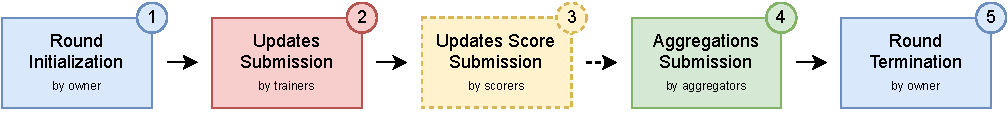
\includegraphics[width=1\textwidth]{graphics/sequence.pdf}
    \caption{BlockLearning Flow}
    \label{fig:blocklearning_steps}
\end{figure}

The framework supports a modular sequential flow represented on \autoref{fig:blocklearning_steps}. The steps are explained below:

\begin{enumerate}
    \item In first place, the owner initializes the round. During the round initialization, depending on the participant selection algorithm, the trainers that will participate may be already defined, or not.
    
    \item In second place, the trainers retrieve the information about the round, such as the global weights from the last round, and train the model using their local data. Then, the trainers submit their updates.
    
    \item In third place, if there is a scoring algorithm enabled, the scorers retrieve the updates and calculate the scores. Then, they submit their scores.
    
    \item In fourth place, the aggregators retrieve the updates and execute the aggregation algorithm and submit the aggregation results.
    
    \item In fifth place, if we are using vertically partitioned data, and depending on the model in use, the trainers may have to confirm back-propagation. Note that this step is tightly connected to the model we will be using for Vertical Federated Learning, which will be introduced later. Nonetheless, it shows how modular the system can be and how steps can be easily added at different points of the flow for different purposes.
    
    \item Finally, the round is marked as terminated by the owner. At this point, the smart contract decides which is the final aggregation for the model based on the submissions by the aggregators.
\end{enumerate}

\subsection{Threat Model}

In the last step of the execution flow, the smart contract decides the final aggregation values based on the submissions by the aggregators. For this, at least 50\% of the aggregators must agree on the same aggregation in order for it to be accepted. Therefore, the framework offers a 50\% threat model.

Even though 50\% is not the ideal threat model, it is a clear improvement compared to regular Federated Learning where the central aggregator is a single point of failure that has to be always available, reliable and trusted. In this framework, an attacker would have to control over 51\% of the aggregators in order to be able to influence the outcome of the aggregation, and therefore, or the training.

In addition, the framework should allow for the threat threshold to be changed. By default, it is 50\%. However, if a user prefers that all aggregators must agree on the same aggregation, they should be able to do so.

\subsection{Structure and Modules}\label{meth:struct_modules}

The framework is divided into three main parts: the smart contracts, the library and the testbed. These are depicted on \autoref{fig:blocklearning_modules} and will be individually explored on the following subsections.

\begin{figure}[!ht]
    \centering
    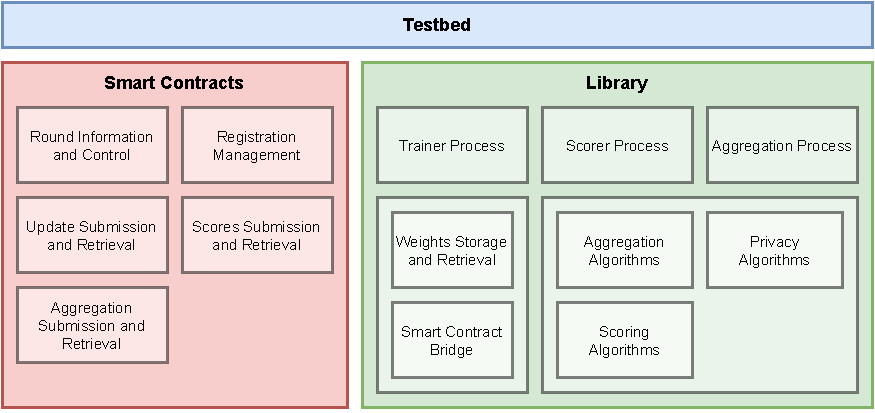
\includegraphics[width=1\textwidth]{graphics/modules.pdf}
    \caption{BlockLearning Structure and Modules}
    \label{fig:blocklearning_modules}
\end{figure}

\subsection{Smart Contracts}\label{meth:smart_contracts}

The first component of the framework is the smart contracts. The smart contracts live on the blockchain and are the main means of communication between clients and servers. In addition, the smart contracts hold information regarding the current status of the round, as well as the updates, scores, aggregations, among others. The smart contracts provide the following functionality:

\begin{itemize}
    \item \textit{Round Information and Control}: the smart contract must provide information on whether the round is ongoing and which phase it is in: scoring, aggregation or termination. It must allow for enough flexibility such that new phases can be added in the future. In addition, it must allow for rounds to be started and marked as terminated. Round phase advancements are defined through pre-defined conditions that, once met, automatically move the round to the next phase. For example, after all updates are received, the smart contract should move to the next phase.
    
    \item \textit{Registration Management}: the smart contract must allow devices to register themselves as trainers, aggregators, or scorers in the system. Regarding the owner, it is automatically assigned to whom deployed the contract. Finally, it should provide information about which devices participate in each round.
    
    \item \textit{Update Submission and Retrieval}: the smart contract must allow trainers to submit their updates, which must include a pointer to the model weights and the amount of data points that were used to train the model. In addition, it can include the training accuracy and testing accuracy for each individual trainer. The submissions must be accessible.
    
    \item \textit{Scores Submission and Retrieval}: the smart contract must allow scorers to submit their scores. It must be possible to know which scorer scored which update and they must be accessible.
    
    \item \textit{Aggregation Submission and Retrieval}: the smart contract must allow aggregators to submit the aggregations, which contain a pointer to the weights. The aggregations must be accessible.
\end{itemize}

\subsection{Library}\label{meth:library}

The second part of the framework is the library. The library encodes the algorithms, utilities and building blocks necessary to write the process that runs on the clients and the servers. It must include:

\begin{itemize}
    \item \textit{Aggregation, Scoring} and \textit{Privacy Algorithms}: provide implementation for aggregation, scoring and privacy algorithms. Each of these categories of algorithm must implement a common interface, such that adding new algorithms is easy and simple and they are interchangeable in the code.
    
    \item \textit{Weights Storage and Retrieval}: utilities to load and store weights on the decentralized storage provider. These must also provide an interface in order to make it easy to change the storage provider by providing a different implementation.
    
    \item \textit{Smart Contract Bridge}: a contract class that provides an interface to the smart contract that lives on the blockchain. With this class, it is possible to call the smart contract functions as if they were local functions.
    
    \item \textit{Trainer, Scorer} and \textit{Aggregator Classes}: a class per each device category. This class must register the devices as their category upon initialization. It must also provide methods to execute the training, scoring and aggregation tasks, respectively.
\end{itemize}

\subsection{Testbed}\label{meth:testbed}

The third part of the framework is the testbed. The testbed provides the platform to conduct the experiments in a reproducible way. It must include:

\begin{itemize}
    \item \textit{Client} and \textit{Server Processes}: scripts that will be run at the clients and the servers, respectively. These scripts will use the library in order to perform the right tasks according to which algorithm is being used.
    
    \item \textit{Federated Learning Setup and Deployment}: scripts and tools to easily deploy the client and server machines in a test environment, such as containers.
    
    \item \textit{Blockchain Setup and Deployment}: scripts and tools to easily deploy the blockchain network in a test environment, as well as deploy the contract to such network.
\end{itemize}

In addition, the testbed must also include tools to collect the required statistics and logs that can be later processed to retrieve the previously discussed metrics.

\section{Client Sampling}\label{meth:client_sampling}

The client sampling, that is, the process of choosing which samples are attributed to which client, varies depending on whether we want to partition the data horizontally, or vertically. The following subsections explain how the data is sampled for each of the data partitions.

\subsection{Horizontal}

As previously explained in \Cref{background:archfl}, in horizontally partition data, different clients have different samples that share the same feature space. In addition, for a distributed system such as this one, it is expected that the clients are both heterogeneous in characteristics, and in data. Therefore, it is safe to assume that the data distribution in a distributed setting is \textit{non-iid}.

To simulate a \textit{non-iid} distribution, both in number of samples, as in number of classes at each client, the Dirichlet distribution can be used \cite{tim, 10.48550/arxiv.2006.07242}. The Dirichlet distribution, $Dir(\alpha)$ is a probability distribution characterized by its parameter $\alpha$, which controls the degree of \textit{non-iid}-ness of the distribution. The higher the $\alpha$, the more identically distributed the data will be. The lower the $\alpha$, the more likely it is for each client to only hold samples of a single class.

For our experiments, $\alpha = 0.1$ is used in the Dirichlet distribution as it yields a realistic \textit{non-iid} distribution \cite{10.48550/arxiv.2006.07242}, where some clients only hold many samples of a few classes, while other clients have few samples of many classes. In addition, each client has, on average $2500$ samples, such that some clients have lower amounts, and others have higher amounts, simulating a \textit{non-iid} distribution in regards to the number of samples at each client.

\subsection{Vertical}\label{subsection:verticalpartitioning}

Vertically partitioned data is significantly different from horizontally partition data, in the sense that the clients share intersecting sample spaces, but different feature spaces. Therefore, it is not possible to simply attribute some samples to some clients, and other sample to other clients. We have to give each client samples of the same sample space, but different features.

The vertical data partition used in this experiment is based on the work done in \cite{10.48550/arxiv.2104.00489}. Firstly, we choose how many sample to assign each client. To have a comparable experiment, we chose the same amount as for the horizontal partitioning, $2500$ samples. This samples are chosen at random, keeping the original data distribution from the original data set. Then, each sample is attributed a unique identifier (ID) that will be used as label when giving the data set to each client. Only the model owner, or server, has access to the true labels. After choosing the IDs, the feature space $F$ is divided into $C$ parts $F_c$, where $C$ is the number of clients. Finally, the features $F_c$, with $c \in C$ are attributed to each one of the clients.

Since the vertical partitioning is more dependent on the data set and ML model in use than the horizontal partitioning, more details are provided in \Cref{chapter:evaluation}.

\section{Experiments}\label{meth:experiments}

The conducted experiments can be divided into six groups, of which five compare how using different types of algorithm impact the system. These five groups can be divided as: consensus algorithms, participant selection algorithms, scoring algorithms, number of clients and privacy degrees. The sixth group of experiments is dedicated to show a proof of concept of how vertical federated learning can be applied to a BFS system.

Even though all experiment groups compare different things, there are certain aspects that are common to all of the experiments. Firstly, all experiments are run for 50 rounds. 50 rounds was chosen such that we can compare the accuracy results to other papers in order to validate if our experiments are within the expected values. Secondly, all experiments are run with 10 servers.

\subsection{Consensus Algorithms}

In the first experiment group, we compare different consensus algorithms in order to analyze their impact, if any, in accuracy, convergence, communication and computation costs. To do so, we execute three experiments with 25 clients, random participants selection and no scoring algorithm. In each experiment, we use a different consensus algorithm: PoA, PoW and QBFT.

\subsection{Participant Selection Algorithms}

In the second experiment group, we compare different participant selection algorithms. Similarly to the previous experiment group, we set the number of clients at 25 and no scoring algorithm. In addition, the consensus algorithm is set to PoA and then we execute two experiments: one using random selection, and the other using a first come first served basis selection.

\subsection{Scoring Algorithms}

In the third experiment group, we compare the different scoring algorithms. To do so, we use the PoA consensus algorithm, 25 clients and random client selection. Then, we run an experiment for each scoring algorithm: BlockFlow, Marginal Gain and Multi-KRUM, as well as without a scoring algorithm.

\subsection{Number of Clients}

In the fourth experiment group, for each of the scoring algorithm, we analyze the impact of the number of clients. The environment settings are the same as for the scoring algorithms, except that we vary the number of clients: 5, 10, 25, 50. These number of clients were decided based on the current literature and on the available resources we have at our disposal to execute the experiments.

\subsection{Privacy Degrees}

In the fifth experiment group, for each of the scoring algorithms, we compare the impact of different privacy degrees. To do so, we have a similar environment to the previous experiment. However, the number of clients is fixed at 25. Then, we vary the privacy degree by setting the $\epsilon$ parameter for the local differential privacy. The privacy degrees tested are none, $\epsilon = 1$ and $\epsilon = 5$, which allows us to test the impact of a high level of privacy, as well as a lower one.

\subsection{Vertical Federated Learning}

In the sixth and last experiment group, we investigate if it is possible to implement and run a Blockchain-based Federated Learning with vertically partitioned data. Two experiments are run for this group with 2 and 4 clients. The low number of clients is due to the nature of the data set and how we partition the data vertically. In addition, this experiment will not include a scoring or participation selection algorithm.

As explained in \Cref{background:archfl}, Vertical Federated Learning systems have an additional step where the Private Set Intersection (PSI) of the client's data sets is calculated. In this work, we assume that the PSI is calculated beforehand and that it is already known to all devices. In future works, it would be interesting to integrate a PSI mechanism into the framework.

\section{Metrics}\label{meth:metrics}

To compare the different experiments, we define a set of metrics regarding to the different aspects we are comparing: execution time, accuracy, communication and computation costs.

To compare execution time, we define two metrics: the \textit{End-to-end (E2E) execution time} and the \textit{Mean Round Execution Time}. The former is defined by the time it takes for an experiment to execute from start to end. The latter is defined by the mean time it takes to complete a round, which can be calculated by dividing the E2E Execution Time by the number of rounds of the experiment.

To compare the blockchain costs, namely the impact of waiting for transactions, we define two metrics: the \textit{Transaction Latency} and the \textit{Transaction Cost}. The former is defined by the time it takes between submitting a transaction and receiving the confirmation. The former is defined by how much it costs to submit a transaction, which is usually some sort of internal currency used by the blockchain platform.

To compare the accuracy, we use a global \textit{Accuracy} metric for the model, where the model owner, that is, the one that initiates the process, has some data set with which they can test the model.

To compare communication costs, we define the \textit{Network Traffic Per Round}. This metric is defined by how much network traffic is necessary per round and it is collected for the client, server and blockchain processes individually. With this, we can take conclusions on how it would affect different types of devices. For example, if there is a high volume of traffic per round at the client process, but the clients have a low network bandwidth, then it is expected for the rounds to take longer on average.

To compare the computation costs, we collect the \textit{RAM Usage} and \textit{CPU Usage}. Similarly to the communication costs, both these metrics are collected at the client, server and blockchain processes. This metrics allows us to compare and visualize how different algorithms impact the computation costs at each process.

The last two metrics are collected at the client, server and blockchain processes in order to be able to differentiate the effects of the different algorithms on the different parts of the system. However, it is important to note that, in practical settings, the server process and the blockchain process run on the same device.
